\documentclass{standalone}

%----------------------------------------------------------------------------------------------%
%                                 Packages and basic declarations
%----------------------------------------------------------------------------------------------%

\usepackage{amsmath}
\usepackage{mathrsfs}
\usepackage{pgf}
\usepackage{tikz}
\usepackage{verbatim}
\usepackage{pgfplots}


\usetikzlibrary{arrows}




%----------------------------------------------------------------------------------------------%
%----------------------------------------------------------------------------------------------%
%                                            DOCUMENT STARTS
%----------------------------------------------------------------------------------------------%
%----------------------------------------------------------------------------------------------%

\begin{document}
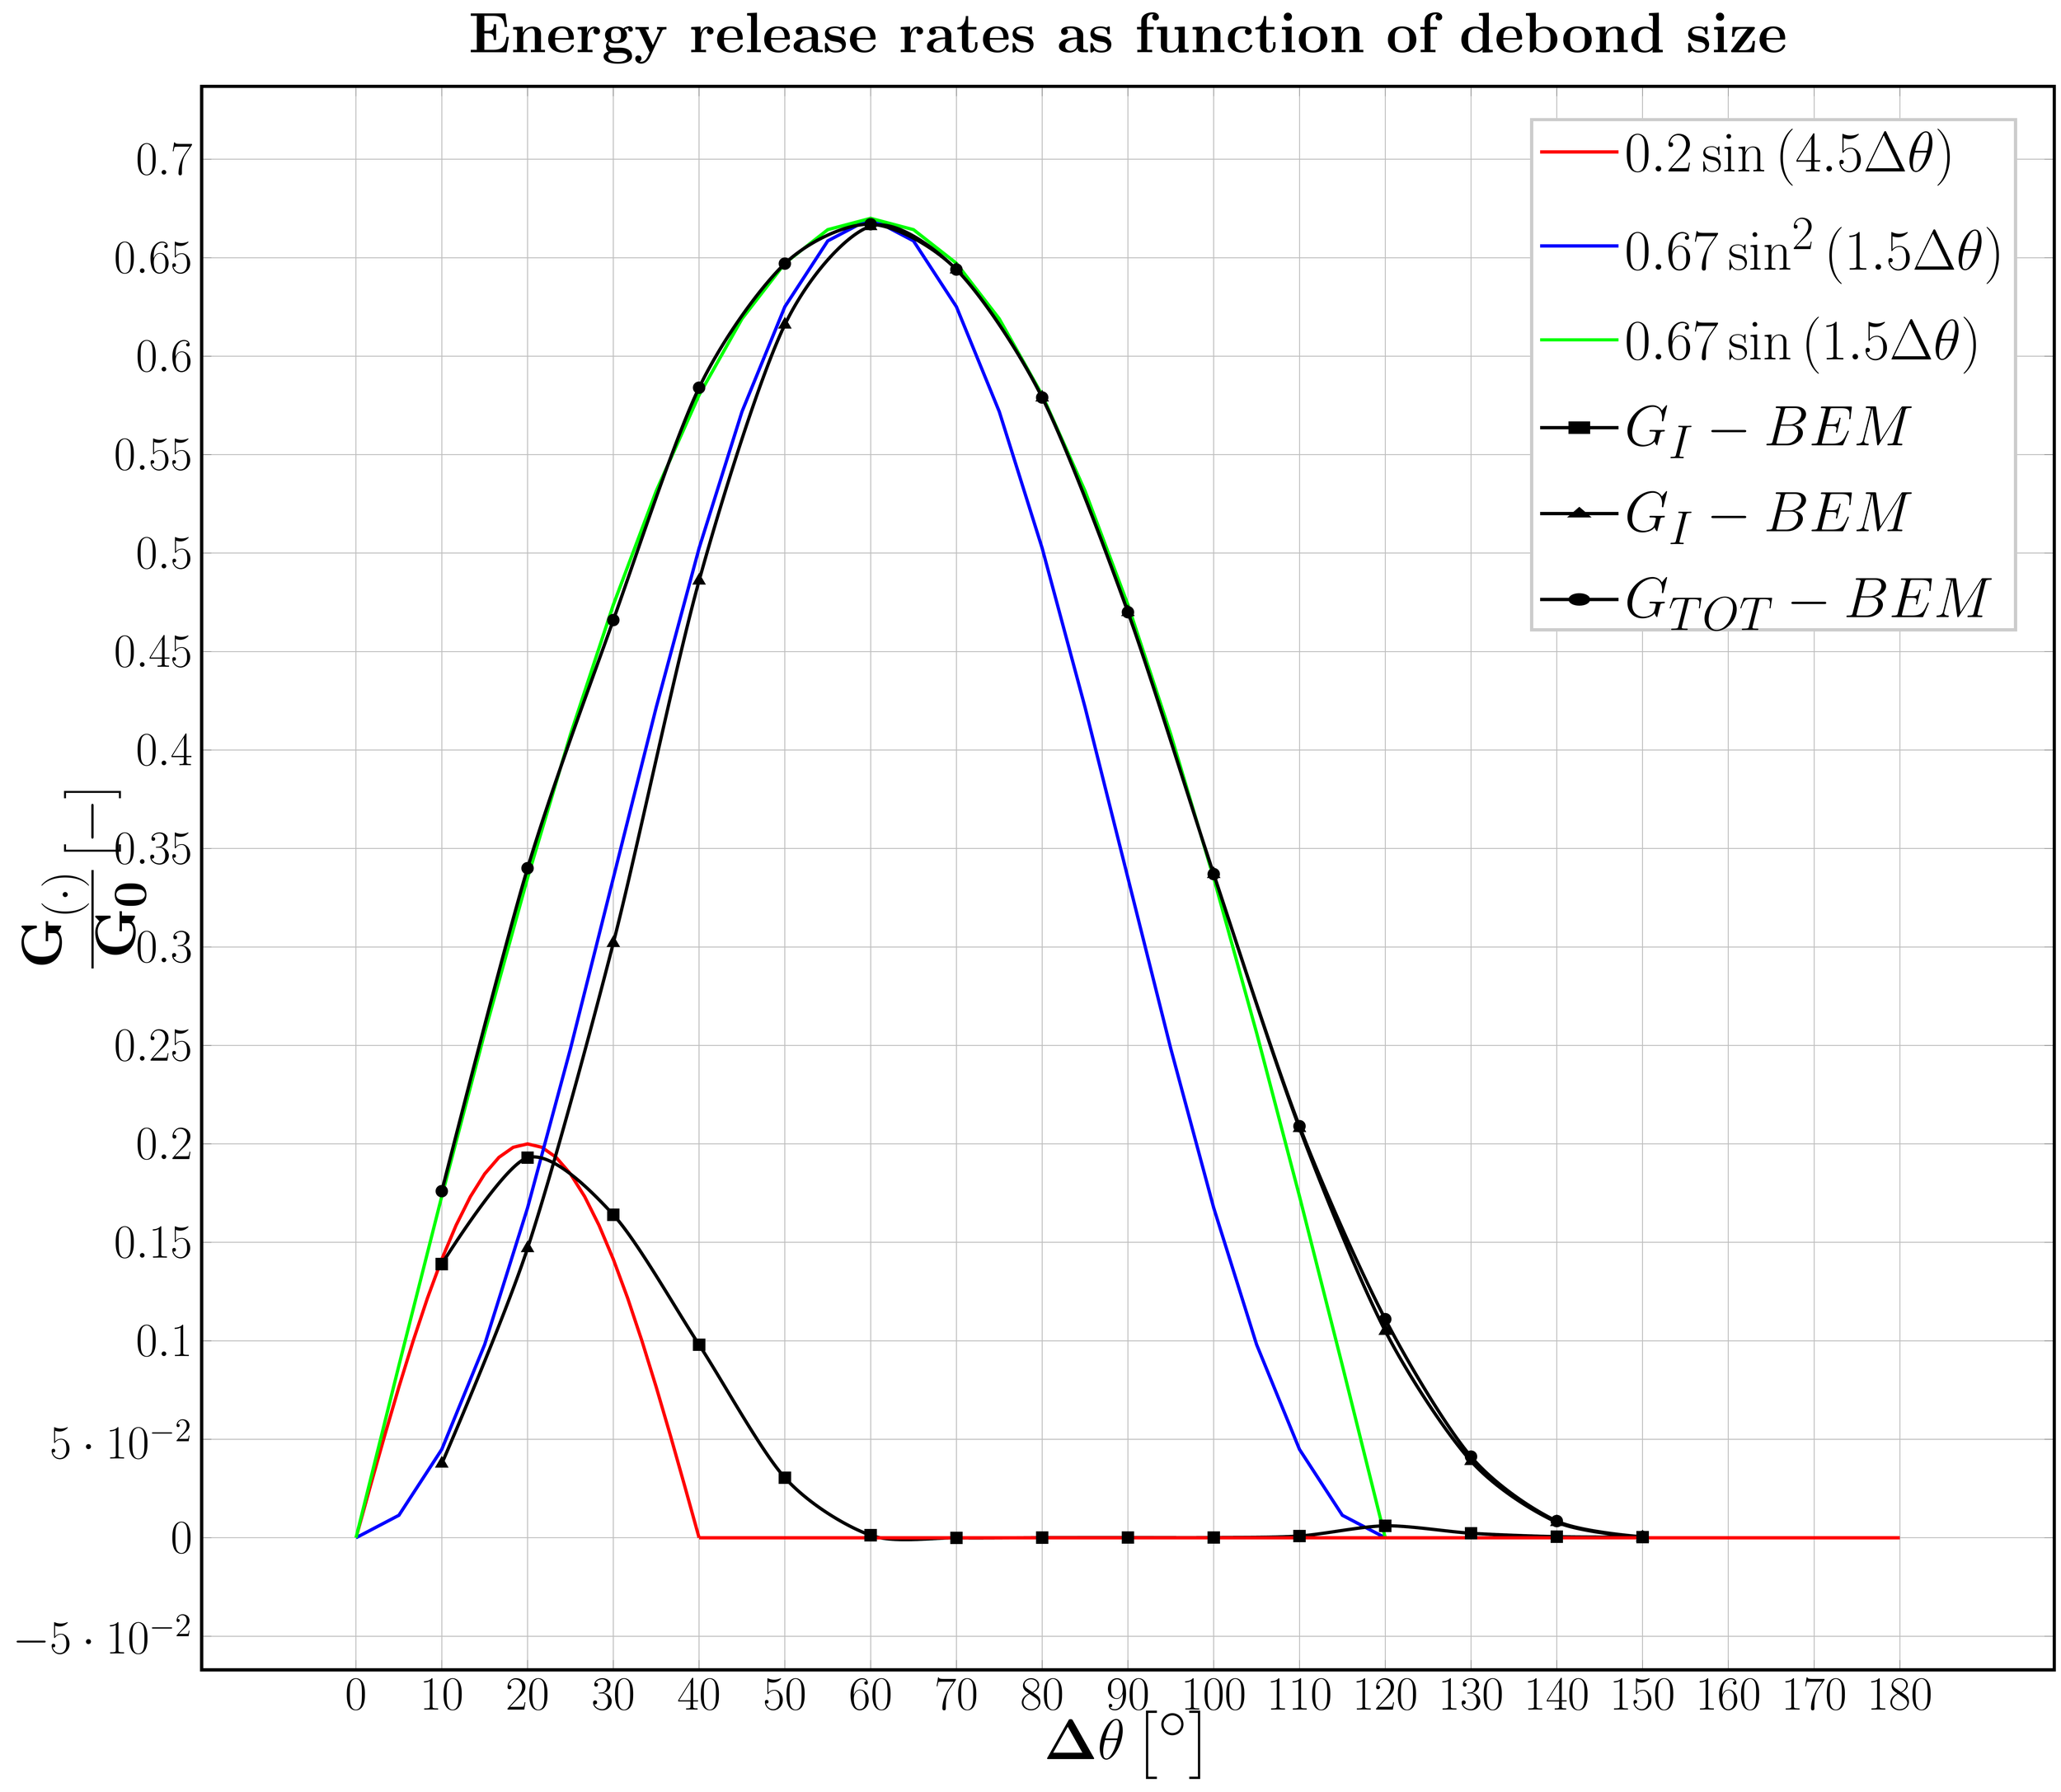
\begin{tikzpicture}[scale=4.5]

\begin{axis}[width=30cm,line width=0.5mm,xmajorgrids,ymajorgrids,xtick={0.0,10.0,20.0,30.0,40.0,50.0,60.0,70.0,80.0,90.0,100.0,110.0,120.0,130.0,140.0,150.0,160.0,170.0,180.0},
title={\bf{Energy release rates as function of debond size}},
title style={font=\fontsize{40}{8}\selectfont},
xlabel style={at={(axis description cs:0.5,-0.02)},anchor=north,font=\fontsize{44}{40}\selectfont},
ylabel style={at={(axis description cs:-0.025,.5)},anchor=south,font=\fontsize{44}{40}\selectfont},
tick label style={font=\huge},
legend style={draw=white!80.0!black,font=\fontsize{28}{24}\selectfont,row sep=15pt},
xlabel={$\mathbf{\Delta\theta\left[^{\circ}\right]}$},ylabel={$\mathbf{\frac{G_{\left(\cdot\right)}}{G_{0}}\left[-\right]}$},
legend image post style={xscale=2},
legend cell align={left}
]
   % \addplot {cos(x)*cos(x)}; 
    \addplot[domain=0:40,red] {0.2*sin(4.5*x)};
    \addplot[domain=0:120,blue] {0.67*sin(1.5*x)*sin(1.5*x)};
    \addplot[domain=0:120,green] {0.67*sin(1.5*x)}; 
   % \addplot[domain=0:40,green] {0.4*sin(2.25*x)*cos(2.25*x)+0.67*sin(1.5*x)*sin(1.5*x)}; 
    % ==========> BEM
\addplot[black,smooth,mark=square*]
table{
10.0000799638 0.139
20.0000438144 0.193
29.9998676461 0.164
40.0002686288 0.098
49.9997304605 0.0305
60.0001314432 0.00127
69.9999586901 -4.79e-05
79.9999225407 6.85e-05
90.0000025045 0.000112
100.000082468 0.000112
110.000046319 0.000895
119.999866736 0.00607
130.000274548 0.00229
139.999726135 0.000552
150.000133948 0.000306
};

\addplot[black,smooth,mark=triangle*]
table{
10.0000799638 0.0376
20.0000438144 0.147
29.9998676461 0.302
40.0002686288 0.486
49.9997304605 0.616
60.0001314432 0.666
69.9999586901 0.644
79.9999225407 0.579
90.0000025045 0.47
100.000082468 0.337
110.000046319 0.208
119.999866736 0.105
130.000274548 0.0389
139.999726135 0.00792
150.000133948 0.000165
};

\addplot[black,smooth,mark=*]
table{
10.0000799638 0.176
20.0000438144 0.34
29.9998676461 0.466
40.0002686288 0.584
49.9997304605 0.647
60.0001314432 0.667
69.9999586901 0.644
79.9999225407 0.579
90.0000025045 0.47
100.000082468 0.337
110.000046319 0.209
119.999866736 0.111
130.000274548 0.0412
139.999726135 0.00847
150.000133948 0.000471
};
    \addplot[domain=40:180,red] {0};
    
    \legend{$0.2\sin\left(4.5\Delta\theta\right)$,$0.67\sin^2\left(1.5\Delta\theta\right)$,$0.67\sin\left(1.5 \Delta\theta\right)$,$G_{I}- BEM$,$G_{I}- BEM$,$G_{TOT}- BEM$}
\end{axis}

\end{tikzpicture}

\end{document}
